%!TEX root = Projeto.tex
\section{Principais conceitos}
Esta dissertação explora o tema da segurança da informação no navegador sob sete aspectos:
\begin{inparaenum}[\bfseries 1)]
	\item dos conceitos básicos de segurança da informação no contexto deste trabalho,
	\item dos fluxos de informação no navegador,
	\item das vulnerabilidades associadas a esses fluxos, caracterizadoras do problema em questão,
	\item do aparato de segurança da informação implementado pelos navegadores e suas deficiências,
	\item dos requisitos para a avaliação da segurança da informação no navegador,
	\item do estado a arte na mitigação de riscos e
	\item dos recursos de programação que embasam a proposta desenvolvida na seção 3 deste trabalho.
\end{inparaenum}
A apresentação desses aspectos é fundamental para a completa compreensão da proposta deste trabalho, seus objetivos e contribuições.

%!TEX root = Projeto.tex
\section{Conceitos básicos}

\subsection{Segurança da informação}
Segundo \cite{ISO2016}, segurança da informação é um processo com os objetivos de ``preservação da confidencialidade, integridade e disponibilidade da informação''. \cite{Foster1998} elabora esses objetivos, descrevendo a confidencialidade como a condição na qual a informação só pode ser acessada pelos agentes autorizados, integridade como a capacidade de proteger a informação contra modificações não autorizadas, e a disponibilidade como a capacidade de garantir acesso à informação quando necessário; \cite{Foster1998} ainda atribui mais duas características a um sistema de segurança da informação: \textit{accountability} como a possibilidade de se atribuir um agente para cada ação ocorrida dentro do sistema, e \textit{assurance} como o grau de confiabilidade na segurança do sistema em relação aos seus objetivos declarados.

Neste trabalho, qualquer definição de segurança da informação será restrita aos sistemas de informação relacionados com a navegação de usuários através da web: provedores de serviço (\textit{sites}, servidores da web), protocolos de comunicação em rede (HTTP, HTTPS, \textit{web sockets}), navegadores (\textit{browsers}) e os ambientes de execução de Javascript embutidos nos navegadores. Isto delimita a área de conhecimento relevante para este trabalho.

%\subsection{Políticas de controle de acesso}
%Segundo \cite{Goguen1982}, uma política de controle de acesso é necessária para que se estabeleçam quais fluxos de dados serão permitidos em um sistema de informação.

\subsection{Modelos de controle de acesso}
Enquanto a definição dos requisitos de segurança da informação estabelece seus objetivos, os modelos definem os sistemas derivados desses objetivos \cite{Goguen1982}. \cite{Foster1998} menciona diferentes modelos de controle de acesso, categorizados de modo amplo como modelos discricionários (DAC -- \textit{discretionary access control}) e mandatórios (MAC -- \textit{mandatory access control}). Modelos discricionários se baseiam na definição dos relacionamentos de segurança entre agentes e objetos em um sistema, como, por exemplo, a política de que um {\script} -- a parte \textit{agente} -- não pode iniciar conexões com domínios diferentes do seu próprio -- a parte \textit{objeto}. Modelos discricionários são os mais comumente utilizados para estabelecer mecanismos de segurança nos navegadores. O campo de atuação desses modelos é limitado aos relacionamentos de segurança estabelecidos, e portanto não podem garantir a segurança da informação quando esta ultrapassa o domínio desses relacionamentos. Isto significa, por exemplo, que dados legitimamente obtidos dentro de regras discricionárias pode ser replicado para um contexto não-seguro sem qualquer impedimento derivado do modelo de segurança.

Modelos mandatórios não atribuem explicitamente as regras de controle de acesso aos objetos e agentes de um sistema. Ao invés disso, estabelecem níveis de confidencialidade utilizados para classificar os participantes do sistema de informação, viabilizando o controle dinâmico do trânsito da informação entre os agentes. Num modelo mandatório, o nível de segurança de um dado impede que ele seja obtido ou modificado por agentes com níveis de segurança mais baixos. O controle do fluxo da informação faz dos MACs modelos mais robustos do que os DACs \cite{Foster1998}.

\subsection{Controle do fluxo de informações}
O controle do fluxo de informações (IFC -- \textit{information flow control}) é um mecanismo que atua, em tempo de execução, nos meios de propagação dos valores entre os espaços de armazenamento de um sistema computacional de modo a impedir fluxos não autorizados dos dados \cite{Denning1976}. IFC é um modelo de controle de acesso do tipo mandatório e baseia-se em \textit{classes de segurança} ``altas'' e ``baixas'', simbolizadas pelas letras \texttt{<h>} e \texttt{<l>}, respectivamente, para indicar graus de confidencialidade das informações e dos seus espaços de armazenamento (\textit{heap}, pilha, redes, dispositivos etc). Operações entre entidades com classes de segurança diferentes, como a cópia do valor de uma variável \texttt{<h>} (confidencial) para a variável \texttt{<l>} (pública), são automaticamente impedidas de prosseguir.

IFC distingue entre fluxos de informação explícitos e implícitos. Um fluxo explícito ocorre quando uma informação classificada como ``alta'' é diretamente copiada para um contexto de classificação ``baixa'', como na listagem de código \ref{Src: jsIFCExplicitFlow}. Em um fluxo implícito, não é a informação em si que transita entre contextos de classificação diferente, mas sim alguma informação derivada dela através da qual seja possível fazer qualquer inferência sobre seu conteúdo. Um exemplo de fluxo implícito encontra-se la listagem \ref{Src: jsIFCImplicitFlow}. Um mecanismo que suporte IFC deve ser capaz de interromper vazamento de informação em ambos os tipos de fluxo.

\lstinputlisting[language=JavaScript,
inputencoding=utf8,
label={Src: jsIFCExplicitFlow},
caption={Vazamento de dados em fluxo explícito de informação}]{codigo/sample02-ifc-implicit.js}

\lstinputlisting[language=JavaScript,
inputencoding=utf8,
label={Src: jsIFCImplicitFlow},
caption={Vazamento de dados em fluxo implícito de informação}]{codigo/sample03-ifc-explicit.js}
%!TEX root = Projeto.tex
\subsection{Fluxos da informação no navegador}

\subsubsection{O navegador e seus subsistemas componentes}
A capacidade que software navegador tem para buscar informação, apresentá-la ao usuário e torná-la interativa é produto da cooperação de subsistemas responsáveis pela comunicação através da rede, a interpretação de código HTML, a representação visual das páginas, o gerenciamento de \poe{caches} e a execução de \scripts{}. Os navegadores divergem na forma de implementação desses subsistemas, mas em geral empregam arquiteturas que enfatizam aspectos não-funcionais como tolerância a falhas, utilização reduzida de recursos e segurança do ambiente de execução. Navegadores como Chrome, Internet Explorer e Safari utilizam separação de processos por aba de navegação \cite{Bright2016} para elevar o nível de isolamento entre as sessões de usuário; Firefox segue essa tendência ao adotar uma arquitetura de múltiplos processos em seus \poe{releases} mais recentes \cite{Nguyen2017}, coordenando até quatro processos de navegação compartilhados entre todas as abas. No âmbito da segurança da informação, a capacidade de execução em múltiplos processos faz com que o navegador isole, em contextos de alta restrição de permissões \poe{(sandboxes)}, quaisquer aplicações web anômalas que tentassem, por meio de \poe{crashes} deliberados, causar instabilidade do navegador ou do sistema operacional pela execução de código em contexto privilegiado \cite{Chromium2018_MPA}.

Em linhas gerais, \citeauthor{HTML5Rocks2011} descreve a colaboração entre seis subsistemas que compõem um navegador moderno, ilustrados pelo diagrama \ref{Fig: diagrama03}, e descritos no quadro \ref{Box: browserComponents}.

\begin{quadro}[h]
	\begin{framed}{\small
	\begin{description}
		\item [Interface do usuário:] expor os elementos interativos de que o usuário dispõe para comandar o navegador, como a barra de endereços, os comandos de navegação (``voltar'', ``avançar'', ``recarregar'') e os comandos de menu do navegador, incluindo os menus de contexto, atalhos, acesso às configurações e às extensões. A janela de interface do usuário hospeda, ainda, o componente de superfície (\poe{canvas}) responsável pela exibição do conteúdo tornado visível (``renderizado'') pelo subsistema Mecanismo do navegador.
		
		\item [Mecanismo do navegador:] comandar o mecanismo de visualização sob a demanda das ações originadas pela interface do usuário e, em resposta a esses comandos, sinalizar mudanças de estado que serão refletidas pela interface de usuário. Exemplo disso é o ciclo de carregamento de páginas da web, que dispara o \poe{download} de recursos de rede, a renderização desses recursos e a atualização da interface de usuário à medida que as etapas do carregamento se sucedem.
		
		\item [Mecanismo de visualização:] ``renderizar'', ou transformar em conteúdo audiovisual, o fluxo de dados transferidos pelo subsistema de acesso à rede. O fluxo de dados carrega informação textual codificada nas linguagens HTML e CSS, e também dados binários em formato de imagem, áudio e vídeo. O mecanismo de visualização pode dar suporte à renderização de dados em formatos não vinculados à HTML, como documentos PDF e arquivos XML.
		
		\item [Acesso à rede:] conectar-se aos provedores de informação indicados por meio de URLs (\poe{uniform resource locators}) e estabelecer fluxos de dados sob diferentes protocolos como HTTP, HTTPS, Web Sockets, WebRTC e FTP.
		
		\item [Persistência de dados:] prover funcionalidades para armazenamento de dados persistentes, incluindo \poe{caches}, \poe{cookies}, suporte ao sistema de arquivos e as APIs para bancos de dados de escala reduzida como \poe{localStorage} e IndexedDB.
		
		\item [Interpretador de Javascript:] compilar e executar código na linguagem Javascript. ``V8'', ``Chakra'' e ``SpiderMonkey'' são os nomes dos subsistemas de interpretação de Javascript empregados pelos navegadores Chrome, Microsoft Edge e Firefox, respectivamente. Os diversos interpretadores aderem às especificações estabelecidas pelo consórcio ECMA sob o padrão ``ECMAScript'', que define a sintaxe e os recursos que devem ser suportados pela linguagem.
	\end{description}}
	\end{framed}
	\caption[Responsabilidades dos subsistemas componentes do navegador]{Responsabilidades dos subsistemas componentes do navegador. Adaptado de \cite{HTML5Rocks2011}}
	\label{Box: browserComponents}
\end{quadro}


%As responsabilidades desses subsistemas são segregadas entre processos distintos, o que eleva a capacidade do navegador de se manter funcional mesmo quando uma determinada página provoca uma falha de execução que termina seu processo hospedeiro \dubious{(e falta ilustrar essa segregação)}

\begin{figure}[h]
	\centering
	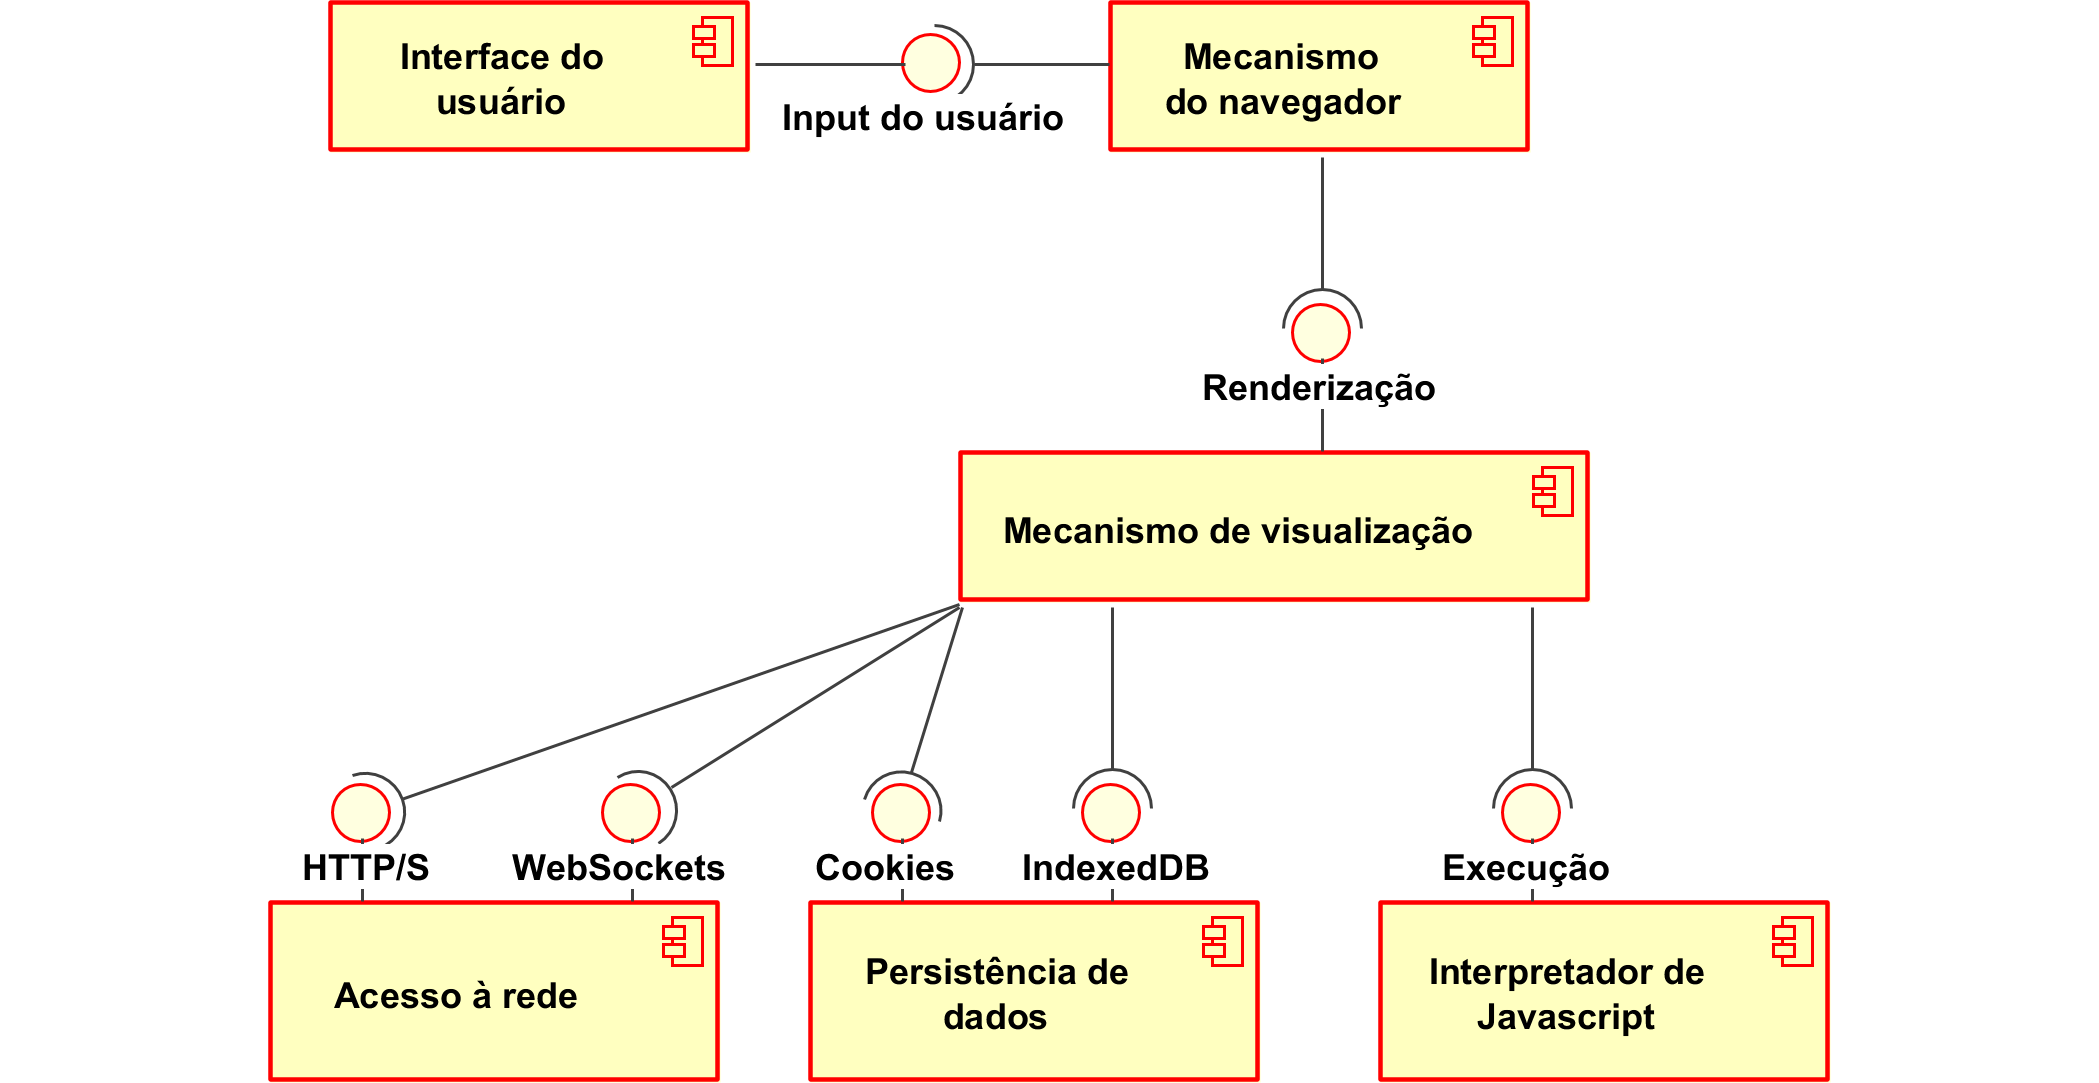
\includegraphics[width=12cm]{diagramas/componentes-navegador.png}
	\label{Fig: diagrama03}
	\caption[Componentes do navegador de código aberto Chromium]{Componentes do navegador de código aberto Chromium. Adaptado de \cite{Chromium2018_MPA, Chromium2018_MPRL, HTML5Rocks2011}}
\end{figure}

% VELHARIAS SEM SUBSTÂNCIA....
% Sob o ponto de vista da segurança da informação, cabem algumas observações:

% \begin{alineas}
% 	\item Os subsistemas do navegador podem apresentar conjuntos próprios de vulnerabilidades, inerentes ao funcionamento e à implementação de cada um;
% 	\item O inter-relacionamento entre esses subsistemas estabelece fluxos de informação que, por sua vez, também podem apresentar vulnerabilidades;
% 	\item Ao longo do tempo, a descoberta de vulnerabilidades e a evolução dos navegadores contribuíram para o estabelecimento de políticas para a segurança na web;
% 	\item A manutenção de certas funcionalidades, necessárias para o funcionamento das aplicações web modernas, comprometeu a capacidade do navegador de se manter imune a todas as vulnerabilidades de vazamento de informação possíveis.
% \end{alineas}

% \subsubsection{Ciclo de vida de uma página da web}

% O ciclo de vida de uma página da web é a sequência de atividades executadas pelo navegador durante os processos de carga, exibição e interação do usuário com o conteúdo visualizado, perdurando até a ação de descarregamento da página, desencadeada pela navegação do usuário ou pelo fechamento da janela do navegador. A informação criada e mantida dentro do ciclo de vida de uma página é volátil, sendo descartada no descarregamento. Para que se torne persistente, a informação precisa ser transmitida em uma requisição HTTP ou armazenada localmente em estruturas como \poe{cookies}, \poe{localStorage} ou IndexedDB, sempre a critério do desenvolvedor da aplicação web de que a página fizer parte.

% É durante o ciclo de vida da página que ocorrem os eventos que levam às vulnerabilidades relevantes para este trabalho. Não apenas a informação requisitada pelo navegador no momento da carga da página, mas também toda informação produzida pela interação do usuário com os elementos de página, compõem o conjunto dados vulneráveis a vazamento. Por meio de disparo de eventos do DOM, um {\script} pode capturar a sequência de ações desempenhadas pelo usuário enquanto este aciona os controles de \poe{mouse}, digita caracteres pelo teclado e efetua rolagem de tela. Mesmo eventos emitidos por ações que não dependam de interação do usuário, como mudanças de estado do DOM e o carregamento de recursos oriundos da rede, podem ser capturados e preservados em uma linha do tempo de acontecimentos que revela toda a experiência do usuário durante o ciclo de vida de uma página.

\subsubsection{Fluxos de informação violadores da privacidade do usuário}

O estudo empírico de \citeauthor{Jang2010}, conduzido em \citeyear{Jang2010} tendo como alvo os 50.000 sites mais visitados do mundo\footnote{O serviço Alexa provê serviços de análise da visitação de sites, sob consulta. \url{https://www.alexa.com/topsites}}, evidenciou uma variedade de fluxos capazes de comprometer a privacidade dos dados de usuário em nos sites \poe{sites} de grande circulação. Os autores descrevem quatro efeitos desses fluxos: roubo de \poe{cookies}, sequestro do endereço corrente (\poe{location hijacking}), espionagem de histórico (\poe{history sniffing}), e observação do comportamento do usuário. Isoladamente ou em conjunto, os fluxos violadores da privacidade podem ser acionados a partir de um único \script{} comprometido, sem que o desenvolvedor do \poe{site} afetado tenha conhecimento ou o poder de neutralizá-los preventivamente.

\begin{alineas}
	\item Roubo de \poe{cookies}. Como qualquer \script{} incorporado, código malicioso tem acesso à toda informação contida na página hospedeira, incluindo informação armazenada em \poe{cookies}, e permissão para enviar essa informação para outros agentes pelo uso de alguma das diversas maneiras de se invocar recursos remotos enumeradas na seção \ref{Secao: Vulnerabilidades_MecanismosPropagacao}. \poe{Cookies} expostos dessa maneira podem ser utilizados para forjar requisições posteriores em nome do usuário, agravando o potencial de comprometimento de informação.
	\item Sequestro do endereço corrente. O endereço URL corrente do navegador é um valor exposto pelo DOM na propriedade |document.location|. Todo código Javascript tem poder de ler e modificar essa propriedade, cuja alteração causa uma imediata carga do endereço especificado. Um \script{} pode aproveitar-se desse comportamento para redirecionar informação contida na página.
	\item Espionagem de histórico. Embora o histórico de navegação propriamente dito, correspondente à sequência de URLs visitadas, não seja exposto pelo DOM, uma forma de ataque conhecida como XSHM \poe{(Cross Site History Manipulation)} \cite{OWASP:XSHM} revela informação suficiente para que seja possível deduzir, por exemplo, se o usuário fez \poe{login} em determinada aplicação-alvo. Um \script{} pode valer-se dessa dedução para emitir requisições mal-intencionadas para esse alvo em nome do usuário corrente.
	\item Observação do comportamento do usuário. \Scripts{} têm a capacidade de registrar código ``ouvinte'' de eventos derivados da interação do usuário com a página web, como movimentos de \poe{mouse}, cliques, acionamento de teclado e rolagem de tela. Essa informação pode ser retransmitida para outros agentes na internet, que poderão acompanhar as ações do usuário em tempo real.
\end{alineas}

\citeauthor{Jang2010} afirmam que as causas que viabilizam a existência desses fluxos são a natureza dinâmica da linguagem Javascript, sua falta de mecanismos de isolamento entre \scripts{}, e a granularidade incoerente das políticas como a SOP.

% \begin{todo}
% Pontos a considerar:

% \begin{alineas}
% 	\item O navegador da web é um cliente da internet.
% 	\item O ciclo de vida de uma página é "curto" (cada página, uma aplicação diferente? um contexto de execução diferente?)
% 	\item Onde está a informação no navegador, e qual sua duração possível?
% 	\begin{alineas}
% 		\item Endereço (URL) corrente
% 		\item Requisição (pode ser da página como de "sub-recursos" como imagens, iframes, scripts, estilos, xhr...)
% 		\item Resposta
% 		\item Estrutura da página (DOM)
% 		\item Eventos do navegador/DOM
% 		\item Closures
% 		\item Pilha de chamadas
% 		\item Extensões do navegador
% 		\item Caches
% 		\item Cookies
% 		\item Local DB
% 		\item Em HTTPS, temos mais fluxos?
% 	\end{alineas}
% \end{alineas}

% Então será possível indicar quais dos fluxos estão protegidos contra vazamento de informação, e como estão. E consequentemente quais fluxos não estão cobertos.
% \end{todo}

%!TEX root = Projeto.tex
\subsection{Vulnerabilidades}
Violações de privacidade são possíveis nos navegadores por causa da natureza dinâmica da linguagem Javascript e de sua ausência de restrições de segurança em tempo de execução \cite{Jang2010}. Seus usuários estão expostos a ataques sutis com objetivos diversos como roubar \textit{cookies} e \textit{tokens} de autorização, redirecionar o navegador para sites falsos (\textit{phishing}), observar o histórico de navegação e rastrear o comportamento do usuário através dos movimentos do ponteiro do mouse e eventos de teclado. Para que {\scripts} mal-intencionados sejam incorporados a páginas benignas, \textit{hackers} fazem uso de vulnerabilidades como \textit{cross-site scripting (XSS)} \cite{OWASP:XSS} e comprometimento de extensões \cite{Heule2015_Most_Dangerous_Code} do navegador.

\begin{todo}
Aqui é preciso apresentar como este problema é caracterizado, nas referências cabíveis. Tudo indica que se trata de um "DOM-based XSS", que eu livremente traduzo como "XSS baseado em DOM" (péssimo). Imagino colocar a definição do OWASP e indicar as classificações do CWE (Common Weaknesses Enumeration) que orbitam em torno do problema.
\end{todo}

\cite{OWASP:DOMXSS} define um ataque denominado ``XSS baseado em DOM'' como a modificação deliberada do modelo de objetos do navegador com o objetivo de influenciar seu ambiente de execução, sem que a visualização da página seja prejudicada ou que o navegador se comporte inesperadamente. Por essa característica, o usuário não percebe que pode haver um ataque em andamento.

\subsubsection{Mecanismos para propagação de informação suportados pelo navegador}
\label{Secao: Vulnerabilidades_MecanismosPropagacao}
\citeinline{Bielova2013} enumera os mecanismos que o navegador oferece para permitir comunicação entre uma aplicação web e outros recursos receptores de dados. A mera possibilidade de comunicação não constitui uma ameaça às aplicações, sendo de fato o meio de se viabilizar as principais funcionalidades do navegador. No entanto, autores de \scripts{} mal intencionados podem tirar proveito dos mecanismos de comunicação para propagar informação sensível.

\paragraph{APIs relevantes} % (fold)
\label{par:apis_relevantes}

\begin{description}
	\item[Objetos do DOM \poe{Core}] Toda a árvore de elementos HTML representada na estrutura do DOM, encabeçada pelo objeto \texttt{window.document}, corresponde à API \poe{core} do DOM. Todos os \scripts{} executando em um determinado domínio têm acesso ao mesmo objeto \texttt{document}. Não havendo garantias sobre as intenções de cada \script{} incorporado, cabe ao autor de uma aplicação web confiar que o comportamento desses \scripts{} não é malicioso do ponto de vista da segurança da informação.
	\item[Domínio] O domínio associado a uma aplicação web é refletido pela propriedade do DOM \texttt{document.domain}, que pode ser modificada por \scripts{}. Um exemplo dessa operação é proporcionado por dois \scripts{}, um executando em um domínio \texttt{a.app.com} e outro no domínio \texttt{b.app.com}. Ambos podem alterar seus domínios de origem para \texttt{app.com}, o que os fará compartilharem o mesmo DOM. Por meio dessa operação os \scripts{} ``relaxam'' a amplitude do domínio relevante para as restrições derivadas da SOP.
\end{description}

% paragraph apis_relevantes (end)


\subsubsection{Compartilhamento do ambiente de execução}
Código \textit{inline} ou {\scripts} baixados pelas páginas da web são executados com os mesmos privilégios e mesmo nível de acesso à estrutura de documento do navegador, o chamado DOM \cite[p. 2-3]{DeRyck2012}, não importando o domínio de origem dos {\scripts}. Uma demonstração do problema pode ser exemplificada na figura \ref{Fig: diagrama01} e listagem de código \ref{Src: webPageMultiOrigin}. Nesse exemplo, um {\script} tido como benigno é incorporado a uma página web a partir de um domínio de CDN (\textit{content delivery network}), diferente daquele da aplicação que efetivamente publica a página. O servidor desse {\script}, pelo protocolo CORS, sinaliza ao navegador que o domínio da página é confiável. O {\script} externo pode, então, iniciar requisições ao seu domínio de origem -- uma consequência desejada pelos autores da página, pois o {\script} depende desse acesso para efetuar suas funções.

\begin{figure}
	\centering
	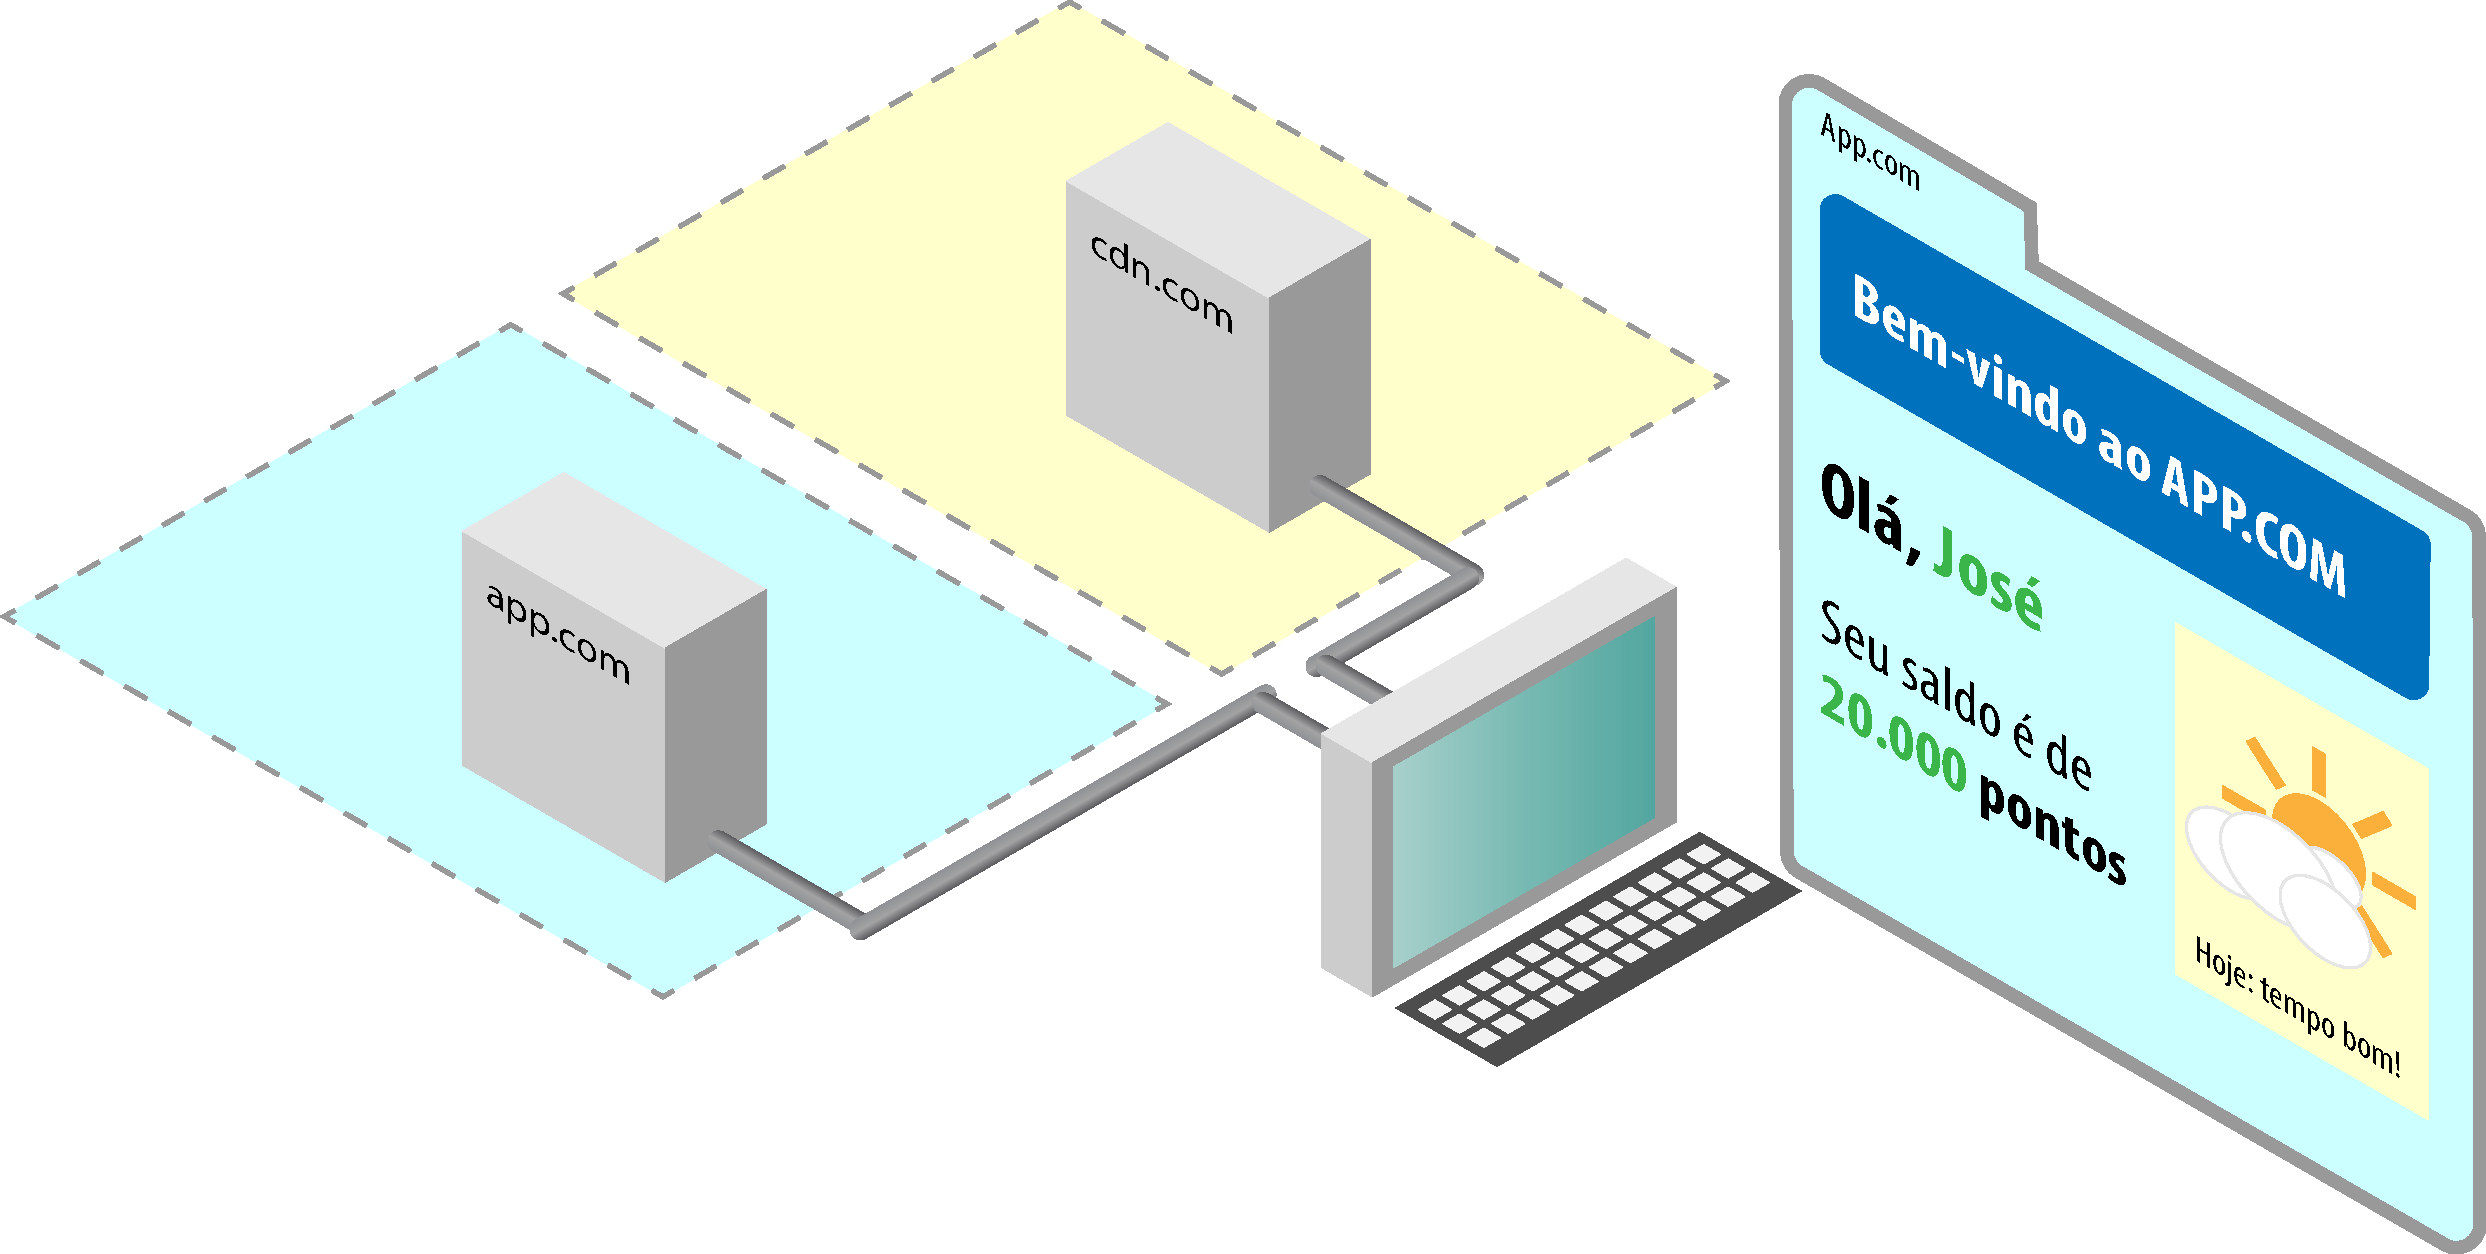
\includegraphics[width=10cm]{diagramas/diagrama01.pdf}
	\caption{Aplicação web composta por conteúdo proveniente de duas origens.}
	\label{Fig: diagrama01}
	
	\lstinputlisting[language=html,
	inputencoding=utf8,
	label={Src: webPageMultiOrigin},
	caption={[Página HTML incorporando {\script} de outra origem]Incorporação de {\script} de outra origem (linha \ref{lstCdnScript})}]{codigo/sample01-leaking-script.html}
\end{figure}

Em momento posterior, o {\script} servido pelos servidores da CDN é substituído por código malicioso que, além de efetuar as funções do {\script} benigno, captura o conteúdo da página armazenado no DOM (figura \ref{Fig: diagrama02}). O {\script} pode buscar informações específicas e potencialmente sensíveis como identificação do usuário, senhas e endereços. Por causa da autorização concedida pelo protocolo CORS, o código mal intencionado tem a chance de transmitir o conteúdo capturado para um serviço anômalo hospedado no mesmo domínio do {\script}.

\begin{figure}
	\centering
	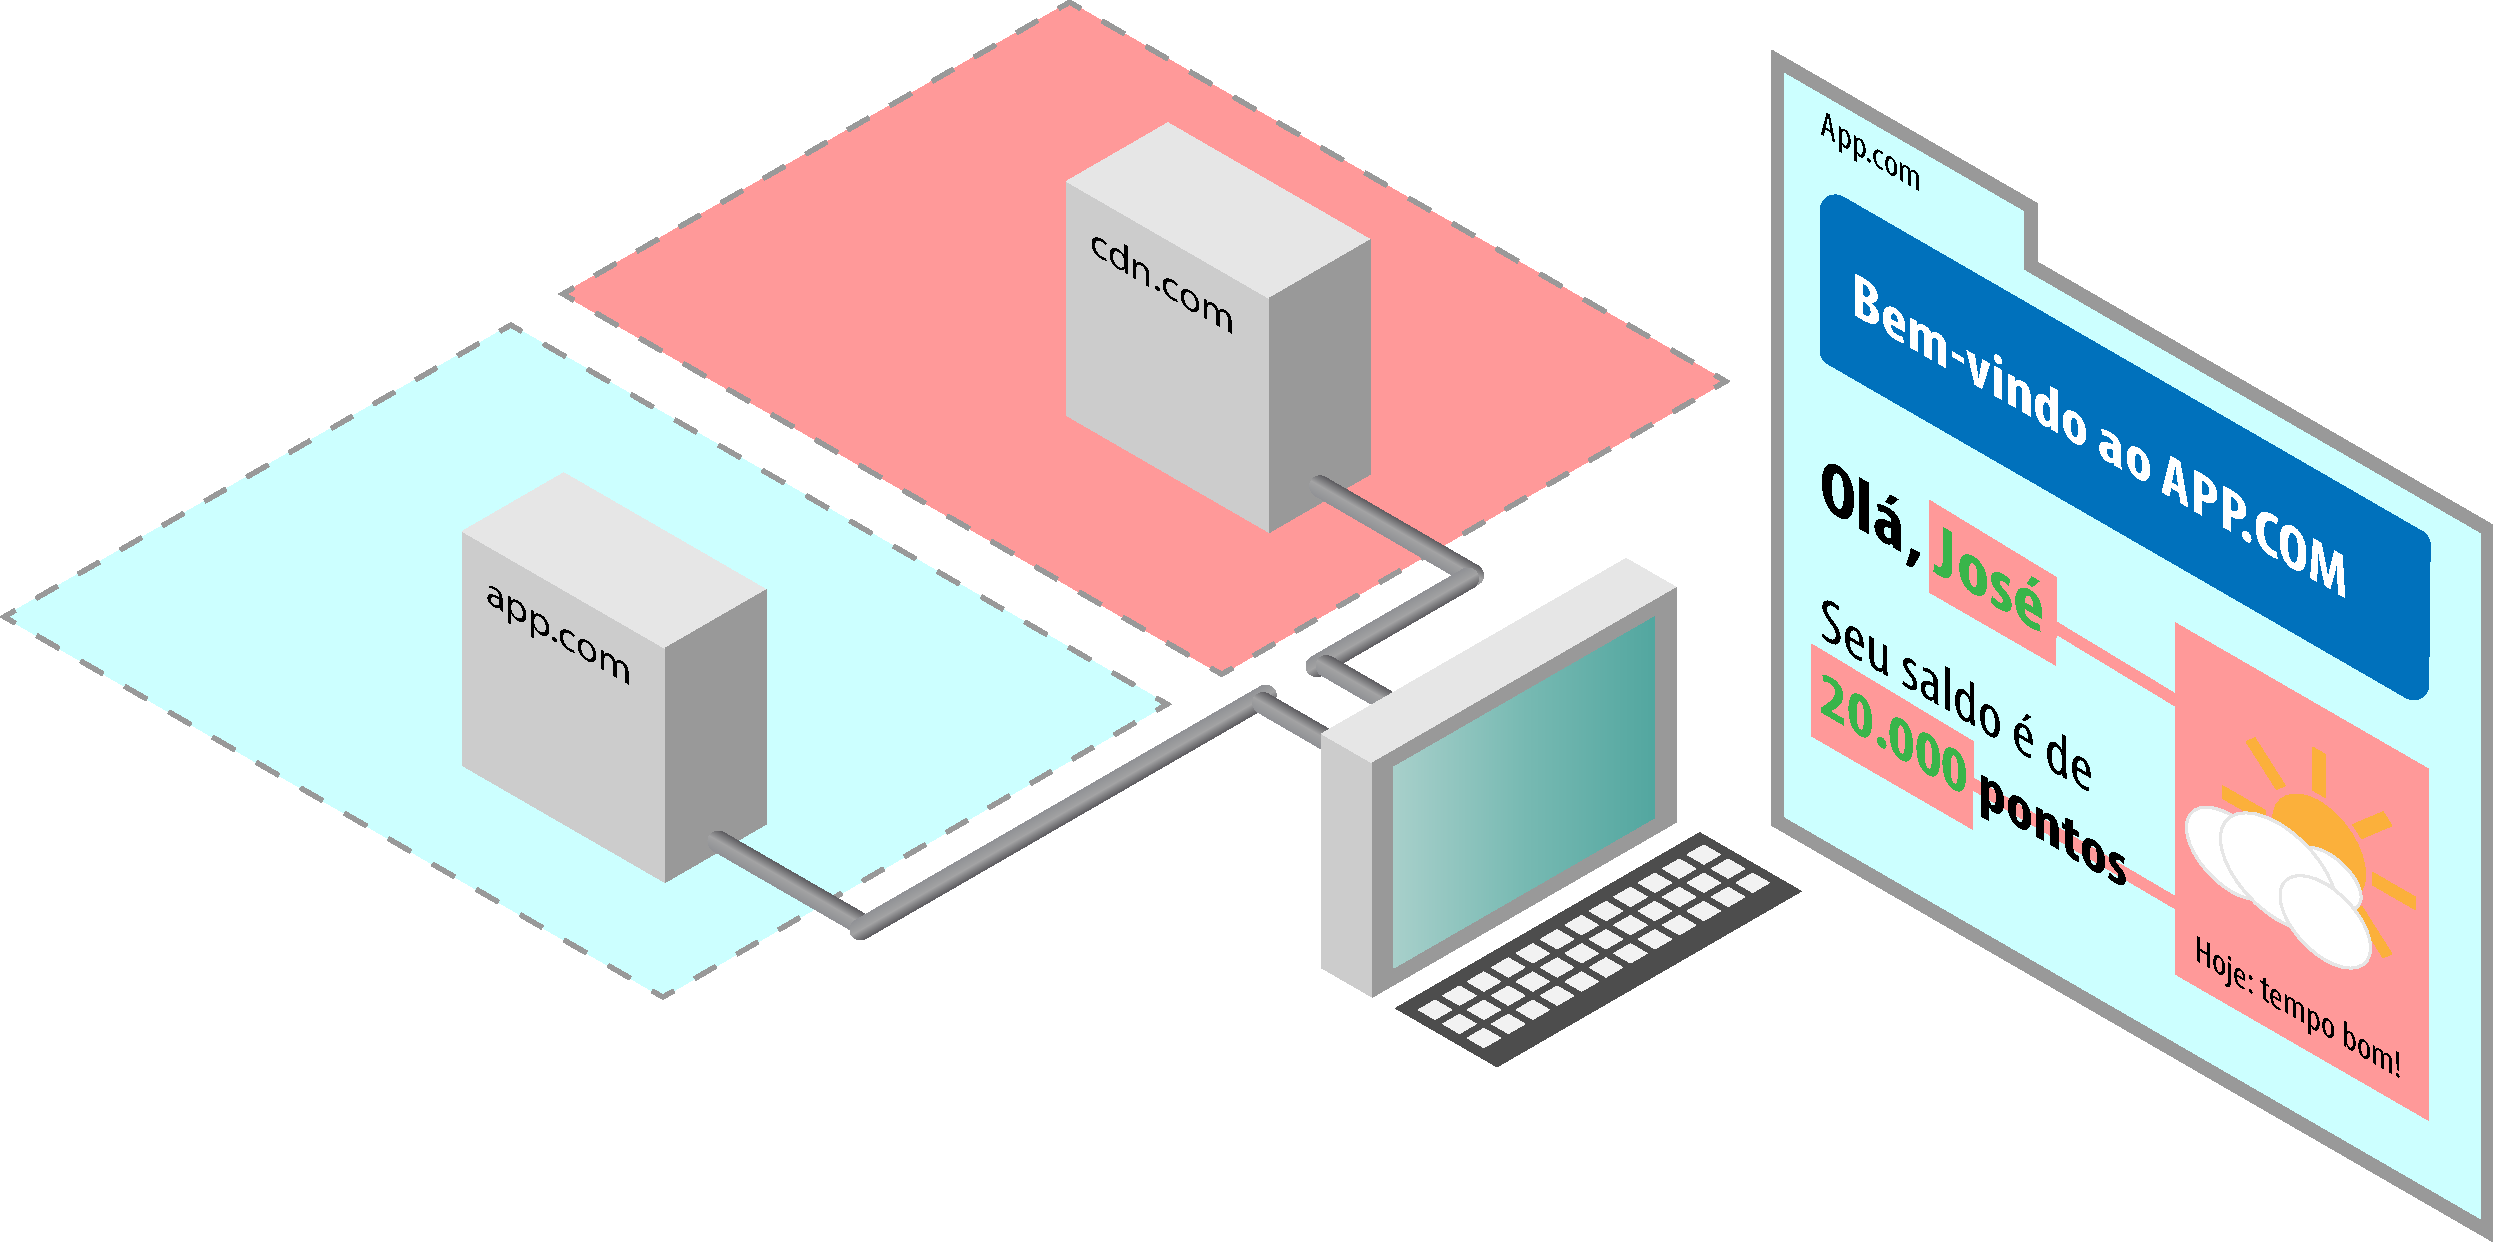
\includegraphics[width=10cm]{diagramas/diagrama02.pdf}
	\caption{Domínio de CDN comprometido, capturando informações do usuário.}
	\label{Fig: diagrama02}
\end{figure}

Acessar, capturar e modificar informações contidas no DOM também são efeitos de extensões do navegador. Mas, diferentemente dos {\scripts} incorporados em páginas, extensões são executadas em modo privilegiado e podem afetar todas as páginas carregadas pelo navegador, não sendo confinadas a domínios específicos. Extensões como as do Google Chrome são publicadas exclusivamente em site específico e protegido, mas não é impossível que o código fonte de extensões seja descaracterizado e publicado pela ação de \textit{hackers} \cite{Spring2017}, afetando a todos os usuários que atualizarem a extensão -- um processo automático por padrão \cite{Google2017}.


\subsubsection{Cross-Site Scripting (XSS)}
Em Javascript, todos os recursos de código carregados dentro de uma mesma página possuem os mesmos privilégios de execução. Ataques do tipo \textit{cross-site scripting} tiram proveito dessa característica para injetar código malicioso em contextos onde seja possível observar e retransmitir informação sigilosa como \textit{cookies} do usuário, endereço do navegador, conteúdo de formulários, ou qualquer outra informação mantida pelo DOM.

O emprego de medidas para prevenção de ataques XSS \cite{OWASP:XSS-CheatSheet} \dubious{(QUAIS?)} não elimina riscos inerentes à tecnologia do navegador. Uma vez que componentes incorporados, como anúncios e \textit{players} de mídia, conseguem carregar {\scripts} tidos como confiáveis dinamicamente, um único trecho de código comprometido pode colocar informações em risco sem qualquer interferência dos dispositivos de segurança.

%\subsubsection{Sobrescrita do DOM} DOM CLOBBERING

%\subsubsection{Scraping} OWASP OAT-011

\subsubsection{Comprometimento de extensões}
Os mecanismos de extensibilidade oferecidos pelos navegadores melhoram a funcionalidade da web para os usuários, e o código de que são feitos é executado com privilégios mais elevados do que o dos {\scripts} incorporados pelos \textit{sites}. Por isso, os usuários precisam confirmar ao navegador que aceitam que uma extensão seja instalada, sendo informados a respeito dos privilégios que a extensão pretende utilizar. O fato de que esse processo precise se repetir a cada vez que uma extensão requisitar de um conjunto de privilégios diferente faz com que os desenvolvedores optem por solicitar, de antemão, uma gama de privilégios maior que a estritamente necessária \cite{Heule2015_Most_Dangerous_Code}.

Uma extensão que tiver sido comprometida (por exemplo, ao usar {\scripts} de terceiros que, por sua vez, tenham sido redirecionados ou adulterados) terá assim poder para ler e transmitir todo o conteúdo carregado e exibido pelo navegador, com o potencial de causar os mesmos efeitos observados em um ataque XSS, mas em escopo e poder aumentados, já que poderiam afetar todas as páginas abertas e todas as APIs publicadas pelo navegador.

\tbc
%!TEX root = Projeto.tex
\subsection{Aparato de segurança da informação implementado pelos navegadores}
% !TeX spellcheck = <none>
%!TEX root = Projeto.tex
\subsection{Requisitos para avaliação da segurança da informação no navegador}

% \begin{todo}
% 	Trazer, da bibliografia, requisitos para avaliação da segurança. Importante estabelecer os critérios para a seleção desses requisitos. Esses requisitos são necessários para o corpo principal do trabalho, mais adiante. Esta seção será enorme.
% \end{todo}

% \tbc
%!TEX root = Projeto.tex
\subsection{Abordagens para mitigação de riscos}

\subsubsection{Políticas padronizadas}

\paragraph{SOP -- Same Origin Policy}
A política de segurança SOP foi estabelecida para que os navegadores conseguissem dar suporte a páginas com conteúdo proveniente de domínios mistos com um mínimo de segurança contra o vazamento de informação entre esses domínios \cite{Hill2016}. Através desta política, os navegadores podem impedir um conjunto de ataques conhecido como \textit{cross-site resource forgery}, em que um domínio tenta instruir o navegador a fazer requisições para outro domínio em nome do usuário \cite{OWASP:CSRF}.

O termo \textit{origem} é intercambiável com a palavra \textit{domínio} e ambos representam, para fins desta política, componentes do endereço de URL associado com cada recurso da web -- a saber, o \textit{protocolo}, o \textit{nome do host} e a \textit{porta TCP} de onde o recurso foi transferido \cite{Barth2011}. Os exemplos a seguir representam recursos de mesma origem:

{
	\small \begin{tabular}{|l|c|l|r|}
		\hline 
		Endereço & Protocolo & Nome do \textit{host} & Porta \\ 
		\hline 
		\texttt{http://exemplo.com/} & http & exemplo.com & 80 \\ 
		\hline 
		\texttt{http://exemplo.com:80/} & http & exemplo.com & 80 \\ 
		\hline 
		\texttt{http://exemplo.com/path/file} & http & exemplo.com & 80 \\ 
		\hline 
	\end{tabular}
}


Os endereços a seguir representam recursos de origens diferentes:

{\small
	\begin{tabular}{|l|c|l|r|}
		\hline 
		Endereço & Protocolo & Nome do \textit{host} & Porta \\ 
		\hline 
		\texttt{http://exemplo.com/} & http & exemplo.com & 80 \\ 
		\hline 
		\texttt{http://exemplo.com:8080/} & http & exemplo.com & 8080 \\ 
		\hline 
		\texttt{http://www.exemplo.com/} & http & www.exemplo.com & 80 \\ 
		\hline 
		\texttt{https://exemplo.com:80/} & https & exemplo.com & 80 \\ 
		\hline
		\texttt{https://exemplo.com/} & https & exemplo.com & 443 \\ 
		\hline
		\texttt{http://exemplo.org/} & http & exemplo.org & 80 \\ 
		\hline
	\end{tabular}
}

Segundo a SOP, as atividades derivadas da inclusão de recursos de origens mistas são categorizadas em três ações \cite{Ruderman2017}:

\begin{alineas}
	\item \textbf{Escrita:} atividades deste tipo instruem o navegador para que ocorra alguma forma de navegação entre páginas, o que inclui a interação com \textit{links}, redirecionamento e submissão de formulários. Em geral SOP não restringe este tipo de ação;
	\item \textbf{Incorporação:} SOP permite que recursos incorporados à página tenham origens mistas. Isto significa que é possível a inclusão de imagens, vídeos, {\scripts} e do elemento \texttt{<iframe>}, entre outros, provenientes de origens mistas e dentro de uma mesma página.
	\item \textbf{Leitura:} atividades de leitura permitiriam que o conteúdo dos recursos carregados pudesse ser consultado entre origens. SOP permite que um subconjunto de funcionalidades de leitura possam ocorrer entre domínios diferentes.
\end{alineas}

Um aspecto importante da SOP é o tratamento dado a {\scripts} incorporados. Quando uma página inclui um {\script} proveniente de outras origens, por exemplo pelo uso de uma CDN (\textit{content distribution network}), esses {\scripts} são executados em contexto da origem do documento em que eles foram incorporados. Isto permite, por exemplo, que \textit{frameworks} populares como jQuery e Angular.js possam ser disponibilizados em CDNs sem perder funcionalidades importantes, como a capacidade de iniciar chamadas assíncronas pela técnica AJAX. Esta concessão da SOP, porém, abre a possibilidade de que esses {\scripts}, se adulterados, executem atividades maliciosas sem impedimentos.

\paragraph{CSP -- Content Security Policy}
CSP foi criada como um complemento à SOP, elevando a capacidade do navegador de servir como plataforma razoavelmente segura para composição de aplicações \textit{mashup} ao estabelecer um protocolo para o compartilhamento de dados entre os componentes da página que residam em domínios diferentes. CSP define um conjunto de diretivas (codificadas como cabeçalhos HTTP) para a definição de \textit{whitelists} -- o conjunto de origens confiáveis -- pelas quais navegador e provedores de conteúdo estabelecem o controle de acesso e o uso permitido de recursos embutidos como {\scripts}, folhas de estilos, imagens e vídeos, entre outros. Através desse protocolo, ataques de XSS que podem ser neutralizados desde que todos os componentes na página sejam aderentes à mesma política de CSP.

\paragraph{CORS -- Cross-Origin Resource Sharing}
Assim como a CSP, o mecanismo CORS \cite{W3C:CORS} complementa a SOP estabelecendo um conjunto de diretivas (cabeçalhos HTTP) para a negociação de acesso via Ajax/XHR a recursos hospedados em domínios diferentes. CORS determina que exista um vínculo de confiança entre navegadores e provedores de conteúdo, dificultando vazamento de informação ao mesmo tempo em que flexibiliza as funcionalidades das APIs. O uso de CORS permite que os autores de componentes e desenvolvedores de aplicações \textit{mashup} determinem o grau de exposição que cada conteúdo pode ter em relação aos outros conteúdos incorporados.

CSP e CORS são recomendações do comitê W3C \cite{W3C:CSP} \cite{W3C:CORS}, sendo incorporados por todos os navegadores relevantes desde 2016 \cite{CanIUse:CSP} \cite{CanIUse:CORS}.

\paragraph{SRI -- Subresource Integrity}



\subsubsection{Abordagens proprietárias}
\begin{todo}
Lembra de alguma? Preciso recordar isto...
\end{todo}


\paragraph{Abordagens experimentais}
\paragraph{JSFLow}
\paragraph{SessionGuard}


\paragraph{Abordagens em processo de padronização}
\paragraph{COWL}
\paragraph{CSP Nível 3}

% !TeX spellcheck = <none>
%!TEX root = Projeto.tex

\section{Shadow DOM}

A evolução do navegador como \textit{host} de aplicações web baseadas em conteúdo misto põe em evidência algumas deficiências relacionadas ao nível de isolamento necessário para que componentes de diferentes origens possam coexistir sem interferirem entre si no que diz respeito ao comportamento e à apresentação esperada, uma vez que a página web é um meio permissivo e sensível a variações sutis como a ordem de carregamento de \scripts{} e folhas de estilo. As listagens \ref{Src: htmlInterference1} e \ref{Src: htmlInterference2} exploram essas fragilidades. Mitigar esses problemas significa que o desenvolvedor precisa ter pleno conhecimento dos efeitos produzidos pelos componentes que ele incorpora a uma página, para então gerenciar esses efeitos de modo que eles produzam a menor quantidade possível de interferências.

A proposta do mecanismo de Shadow DOM é implementar uma forma padronizada para que o próprio navegador minimize as interferências entre componentes que, de outra forma, iriam causar colisões de nome dos estilos e \scripts{}. A utilização de Shadow DOMs faz com que o modelo de objetos em uma página isole determinadas regiões do DOM em \textit{shadow roots} completamente independentes. Assim, interferências como as observadas em \ref{Src: htmlInterference1} e \ref{Src: htmlInterference2} deixam de existir, como demonstrado nas listagens \ref{Src: htmlNoInterference1} e \ref{Src: htmlNoInterference2}. Shadow DOM, \dubious{proposta em xx/201x,} é implementada pelos navegadores Chrome, Opera e Safari, com suporte planejado para os navegadores Firefox e Microsoft Edge \dubious{para os próximos meses}.


